\section{Setting up the System}

The initial positions and velocities of the three stars are chosen such as they correspond to the orbital parameters given in \cref{tab:system_orbit_param}. The inclination, $i$, longitude of the ascending note $\Omega$, and argument of periastron, $\omega$ of the inner orbit relative to the outer orbit define the orientation of the inner orbit with respect to the outer orbit.

The mutual inclination is expected to have the greatest influence on mass transfer among the three factors determining the orientation, thus its a free parameter to be explored. Additionally, I assume that  $\Omega=0^{\circ}$, effectively the line of nodes corresponds to the line connecting the inner binary components and $\omega= 90^{\circ}$. The effective potential of $\xi$ Tau corresponding to the initial configuration of the system is depicted in \cref{fig:triple_equop}.
\begin{figure}[H]
    \centering
    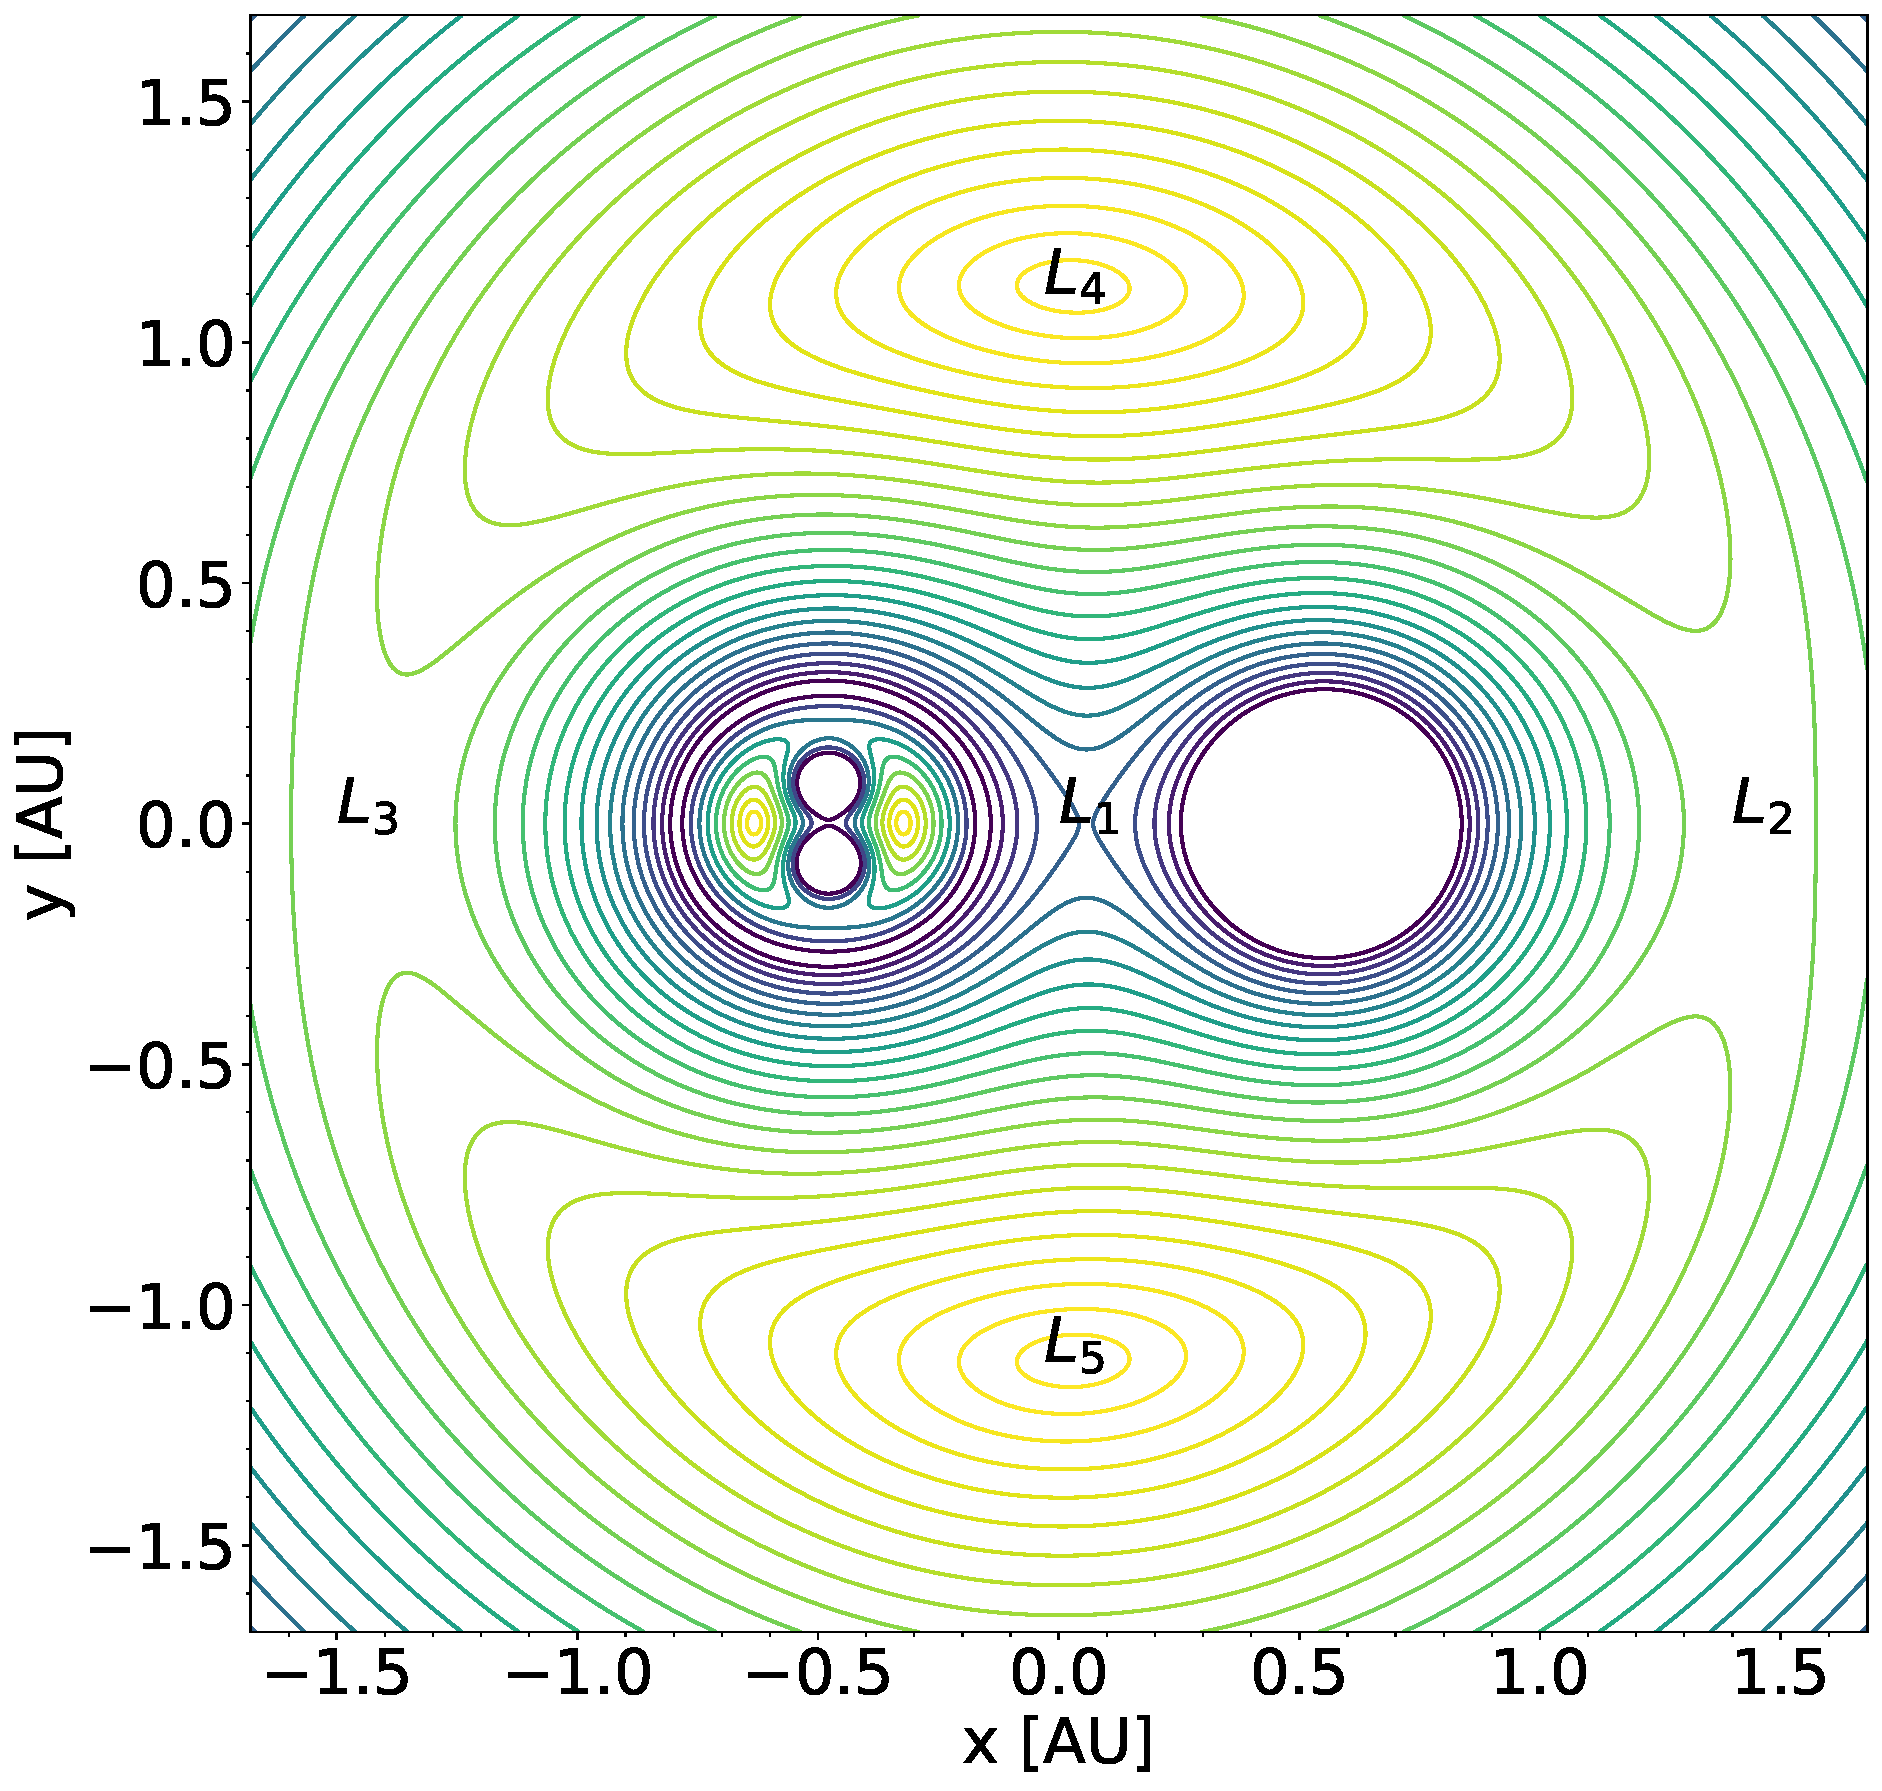
\includegraphics[width=0.9\textwidth]{Thesis/graphs/triple_equop.pdf}
    \caption{Contour plot of $\xi$ Tau's effective potential. The five Lagrangian points of the outer orbit are indicated as $L_1, L_2, L_3, L_4$ and $L_5$. I create this plot using the Hermite integrator which is part of  AMUSE \citep{hut1995building}.}
    \label{fig:triple_equop}
\end{figure}

After relaxing the 3D hydrodynamical model for $t_{relax} =10 t_{dyn}$, I have successfully created a fairly stable model, which represents the outer star. I now replace the outer star, which was a point mass until this point, with the 3D hydrodynamical model.

